\documentclass[../main.tex]{subfiles}

\begin{document}

\chapter{Soft Tissue Engineering}

\section{Stress \& strain in large deformations}

\subsection{Kinematics}

\begin{itemize}
    \item Mapping function 
    \begin{align}
        \vec{x} = \underline{\varphi}(\vec{X},t)
    \end{align}
    \item Displacement function
    \begin{align}
        \vec{x} = \vec{X} + \underline{U}(\vec{X},t)
    \end{align}
    \item The deformation gradient tensor
    \begin{align}
        d\vec{x} = \textbf{F}(X,t)d\vec{X} \Rightarrow \textbf{F} = \frac{\partial \vec{x}}{\partial \vec{X}} = \frac{\partial \underline{\varphi}}{\partial \vec{X}}
    \end{align}
    \item Volume transformation
    \begin{align}
        dv = \det(\textbf{F})dV=JdV
    \end{align}
    \item Surface transformation: Nanson's Formula
    \begin{align}
        \vec{n}ds = J\textbf{F}^{-\top}\vec{N}dS
    \end{align}
    \item Polar decomposition
    \begin{align}
        \textbf{F} = \textbf{R}\textbf{U} = \textbf{V}\textbf{R} \\
        \Rightarrow \textbf{U}^2 = \textbf{F}^{\top}\textbf{F} = \textbf{C}\\
        \Rightarrow \textbf{V}^2 = \textbf{F}\textbf{F}^{\top} = \textbf{B}
    \end{align}
\end{itemize}

\subsection{Strain}

\begin{itemize}
    \item Nominal strain, Biot strain or Engineering strain
    \begin{align}
        \textbf{e} = \textbf{U} - \textbf{I}
    \end{align}
    \item Green-Lagrange strain
    \begin{align}
        \textbf{E} = \frac{1}{2}(\textbf{F}^{\top}\textbf{F} - \textbf{I}) = \frac{1}{2}(\textbf{U}^2 - \textbf{I})
    \end{align}
    \item Euler-Almansi strain
    \begin{align}
        \textbf{A} = \frac{1}{2}(\textbf{I}-\textbf{V}^{-2})
    \end{align}
    \item True strain or logarithmic strain
    \begin{align}
        \bm{\varepsilon} = \ln(\textbf{U})
    \end{align}
\end{itemize}

\subsection{Stress}

\begin{itemize}
    \item True stress or Cauchy stress
    \begin{align}
        \bm{\sigma}^{\top} = \frac{d\vec{f}}{\vec{n}dS}
    \end{align}
    \item 1PK: first Piola Kirchoff stress (Nominal stress or Engineering stress)
    \begin{align}
        \textbf{P} = \frac{d\vec{f}}{\vec{N}dS_0}
    \end{align}
    \item 2PK: second Piola Kirchoff stress
    \begin{align}
        \textbf{S}^{\top} = \frac{\textbf{F}^{-1}d\vec{f}}{\vec{N}dS_0}
    \end{align}
    \item Swithcing between stresses:
    \begingroup
        %\setlength{\tabcolsep}{20pt}
        \renewcommand{\arraystretch}{1.5}
        \begin{tabular}{c|ccc}
             & $\bm{\sigma}$ & \textbf{P} & \textbf{S} \\
            \hline
            $\bm{\sigma}$ & $\bm{\sigma}$ & $J^{-1}\textbf{P}\textbf{F}^{\top}$ & $J^{-1}\textbf{F}\textbf{S}\textbf{F}^{\top}$\\
            \textbf{P} & $J\bm{\sigma}\textbf{F}^{\top}$ & \textbf{P} & \textbf{F}\textbf{S}\\
            \textbf{S} & $J\textbf{F}^{-1}\bm{\sigma}\textbf{F}^{-\top}$ & $\textbf{F}^{-1}\textbf{P}$ & \textbf{S} \\
        \end{tabular}
    \endgroup
\end{itemize}

\section{Constitutive modeling}

The most general form:
\begin{equation}
    \bm{\sigma}(t) = \mathcal{F}_{\tau \leq t}\{\textbf{F}(\tau)\}
\end{equation}

\subsection{Hyperelasticity}

Strain energy density function $\Psi$ related to 2PK
\begin{equation} 
    \textbf{S} = \frac{\partial \Psi}{\partial \textbf{E}} = 2\frac{\partial \Psi}{\partial \textbf{C}}
\end{equation}
Strain energy density function related to Cauchy stress
\begin{equation}
    \bm{\sigma} = \frac{1}{J}\frac{\partial \Psi}{\partial \textbf{F}}\textbf{F}^{\top}
\end{equation}
Small strain - linear elasticity (using Hooke's law)
\begin{equation}
    \Psi_{\text{elastic}} = \frac{E\varepsilon^2}{2}
\end{equation}

\subsection{Isotropic hyperelastic materials}

Right Cauchy-Green Tensor (with $\lambda_i$ the PRICIPAL stretches)
\begin{equation}
    \textbf{C} = \left[\begin{matrix}
        \lambda_1^2 & 0 & 0 \\
        0 & \lambda_2^2 & 0 \\
        0 & 0 & \lambda_3^2
    \end{matrix}\right]
\end{equation}
with invariants:
\begin{align}
    I_1 & = \text{tr}(\textbf{C}) = \lambda_1^2 + \lambda_2^2 + \lambda_3^2\\
    I_2 & = \frac{1}{2}[\text{tr}(\textbf{C})^2 - \text{tr}(\textbf{C}^2)] = \lambda_1^2\lambda_2^2 + \lambda_1^2\lambda_3^2 + \lambda_2^2\lambda_3^2 \\
    I_3 & = \det(\textbf{C}) = \lambda_1^2\lambda_2^2\lambda_3^2 = J^2
\end{align}
Some forms of isotropic SEDFs
\begin{itemize}
    \item Generalized Ogden
    \begin{equation}
        \Psi = \sum^N_{p=1}\frac{\mu_p}{\alpha_p}(\lambda_1^{\alpha_p} + \lambda_2^{\alpha_p} + \lambda_3^{\alpha_p} - 3)
    \end{equation}
    \item Neo-Hookean ($N=1$, $\alpha_1=2$)
    \begin{equation}
        \psi = c_1(I_1 - 3)
    \end{equation}
    \item Mooney-Rivlin ($N = 2$, $\alpha_1=2$, $\alpha_2=-2$)
    \begin{equation}
        \psi = c_1(I_1 - 3) + c_2(\lambda_1^{-2} + \lambda_2^{-2} + \lambda_3^{-2} - 3)
    \end{equation}
\end{itemize}

\subsection{Incompressibility}

Consider as SEDF
\begin{equation}
    \Psi_{\text{tot}} = \Psi(\textbf{F}) - p(J-1)
\end{equation}
the 2PK stress becomes
\begin{equation}
    S=2\left(\frac{\partial \Psi}{\partial \textbf{C}} - p \frac{J}{2}\textbf{C}^{-\top}\right)
\end{equation}
hence the Cauchy stress takes the following form
\begin{equation}
    \bm{\sigma} = \frac{2}{J}<textbf{F}\frac{\partial \Psi}{\partial \textbf{C}}\textbf{F}^{\top} - p \textbf{I}
\end{equation}
Using the Neohookean SEDF gives
\begin{equation}
    \bm{\sigma} = 2c_1\textbf{B} - p \textbf{I} = -p_h\textbf{I}
\end{equation}

\subsection{The NeoHookean material formulation}

\begin{equation}
    \bm{\sigma}_{\text{NH}} = \frac{2}{J}c_1\textbf{B}
\end{equation}

\subsection{Anisotropic material formulations}

Fiber vector
\begin{align}
    \vec{M} \in [\vec{a}_0, \vec{b}_0, \vec{c}_0, \vec{d}_0], \vec{b}_0 = [0,\cos\theta,\sin\theta]\\
    \vec{m} = \textbf{F}\vec{M}
\end{align}
with Pseudo-invariants (introduced in the SEDF)
\begin{align}
    I_4 = \lambda^2 = \vec{M}\textbf{F}^{\top}\textbf{F}\vec{M} = \vec{M}\textbf{C}\vec{M}\\
    I_5 = \vec{M}\textbf{C}^2\vec{M}
\end{align}
SEDF decomposition per tissue constituent (with example tissue)
\begin{equation}
    \Psi_{\text{tot}} = \Psi_{\text{elastin}} + \Psi_{\text{collagen}} + \Psi_{\text{smooth muscle cells}} + ...
\end{equation}
The Gasser Ogden Holzapfel (GOH) material model
\begin{align}
    \Psi_{\text{tot}} &= \Psi_{\text{mat}} + \Psi_{\text{fib}_1} + \Psi_{\text{fib}_2} + p(J-1)\\
    \Psi_{\text{mat}} &= c_1(I_1-3)\\
    \Psi_{\text{fib}_i} &= \frac{k_1}{2k_2}\left(\exp[k_2(I_i^*-1)^2]-1\right)\\
    & I_i^* = \kappa I_1 + (1-3\kappa)I_i,\\
    & I_i = \vec{M}_i\textbf{C}\vec{M}_i \left(= \lambda_{\theta}^2\cos^2\alpha_i+\lambda_z^2\sin^2\alpha_i\right),\;\; i=4, 6
\end{align}

\section{Mechanical testing \& parameter fitting}

General optimization problem
\begin{equation}
    \min(\textbf{S}_{\text{mod}}-\textbf{S}_{\text{exp}})
\end{equation}

\subsection{Uniaxial tensile testing}

\subsection{Biaxial tensile testing}

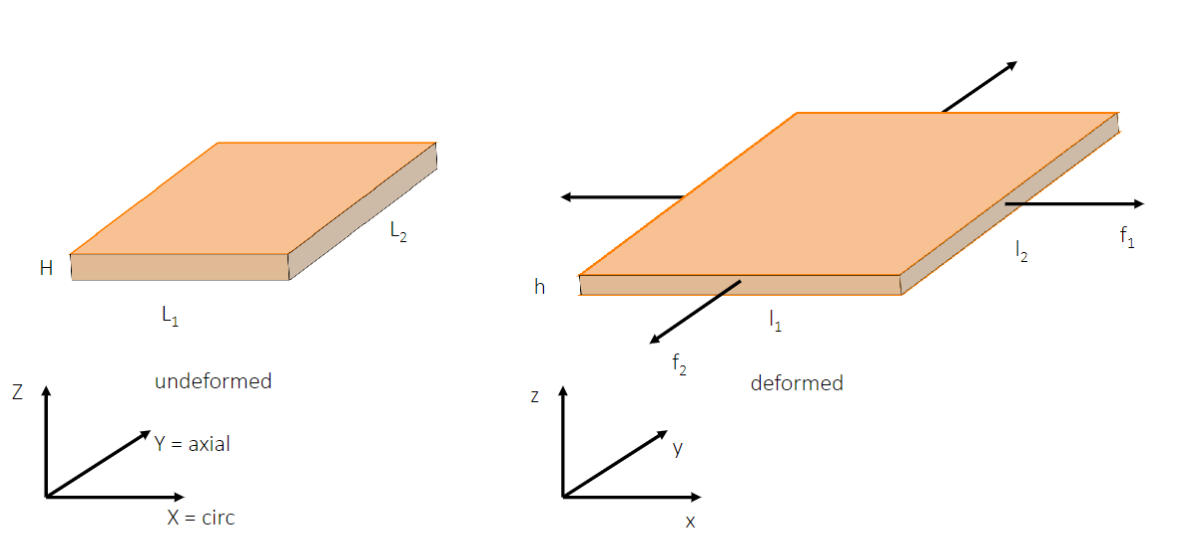
\includegraphics[scale=0.5]{biaxtest.png}

\begin{align}
    \textbf{F} &= \left[\begin{matrix}
        \frac{l_2}{L_2} & 0 & 0 \\
        0 & \frac{l_1}{L_1} & 0 \\
        0 & 0 & \frac{h}{H} \\
    \end{matrix}\right] \\
    \textbf{P} &= \left[\begin{matrix}
        \frac{f_1}{L_2H} & 0 & 0 \\
        0 & \frac{f_2}{L_1H} & 0 \\
        0 & 0 & 0 \\
    \end{matrix}\right] \\
\end{align}

optimization problem (with input data $RF_i$ and \textbf{F}):
\begin{align}
    P_{ij}^{\text{exp}} &= \frac{RF_i}{A_j} \\
    S_{ij}^{\text{mod}} &= 2\frac{\partial\Psi(\textbf{F})}{\partial C_{ij}},\;\; P_{ij}^{\text{mod}} = F_{ik}P_{kj}^{\text{mod}}\\
    &\min_{pars}\sum_i\sum_j\left(P_{ij}^{\text{mod}}-P_{ij}^{\text{exp}}\right)^2
\end{align}

\subsection{Extenson-inflation testing}

Optimization problem:
\begin{itemize}
    \item[$\rightarrow$] Perform Mechanical experiment
    \begin{itemize}
        \item Impose pressure and axial stretch: $p_i$ and $\lambda_z$
        \item Measure axial force and diameter: $f_{zz}$ and $d_o$
    \end{itemize}
    \item[$\rightarrow$] Calculate model pressure
    \begin{itemize}
        \item Model pressure: $P = \int_{r_i}^{r_o} (\sigma_{\theta\theta} - \sigma_{rr})\frac{dr}{r}$
        \item Model axial force: $f_z = 2\pi\int_{r_i}^{r_o}\sigma_{zz}rdr$
    \end{itemize}
    \item[$\rightarrow$] Minimize objective function
    \begin{equation}
        \min_{pars}\left((P^{\text{mod}}-P^{\text{exp}})^2; (f_z^{\text{mod}}-f_z^{\text{exp}})^2\right)
    \end{equation}
\end{itemize}

\subsection{Strain mapping through Digital Image Correlation}

Optimization problem:
\begin{itemize}
    \item[$\rightarrow$] Mechanical experiment: $RF_i$ and $\textbf{F}^{\text{exp}}$
    \item[$\rightarrow$] Run FE simulation:
    \begin{itemize}
        \item input: $RF_i$
        \item output: $\textbf{F}^{\text{mod}}$
    \end{itemize}
    \item[$\rightarrow$] Minimize objective function
    \begin{equation}
        \min_{pars}\sum_i\sum_j\left(\textbf{F}^{\text{mod}}-\textbf{F}^{\text{exp}}\right)^2
    \end{equation}
\end{itemize}

\section{In vivo wall stress estimation}

Calculating the Cauchy stress:
\begin{align}
    \bm{\sigma} &= 2c_1\textbf{B} + \sum_{i=4,6}\left[2k_1E_i\exp(k_2E_i^2)(\kappa\textbf{B}+(1-3\kappa)\vec{m}_i\otimes\vec{m}_i)\right] - p\textbf{I} \\
    \textbf{B} &= \textbf{F}\textbf{F}^{\top}, E_i = I^*_i - 1, \;\; \vec{m}_i = \textbf{F}\vec{M}_i\\
    \textbf{F} &= \left[\begin{matrix}
        1/(\lambda_{\theta}\lambda_z) & 0 & 0 \\
        0 & \lambda_{\theta} & 0 \\
        0 & 0 & \lambda_z
    \end{matrix}\right]
\end{align}

\subsection{Laplace's law for thin-walled tubes}

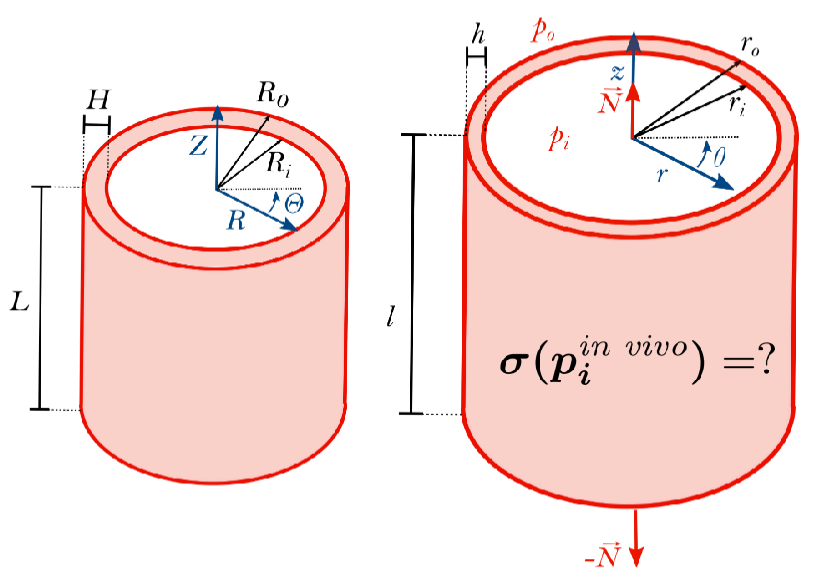
\includegraphics[scale=0.5]{cylindricaltissue.png}

The deformation gradient tensor is givan as
\begin{align}
    \textbf{F} = \left[\begin{matrix}
        1/(\lambda_{\theta}\lambda_z) & 0 & 0 \\
        0 & \lambda_{\theta} & 0 \\
        0 & 0 & \lambda_z
    \end{matrix}\right]
\end{align}
with corresponding stresses
\begin{align}
    \langle \sigma_{rr} \rangle &= -\frac{P}{2} \\
    \langle \sigma_{\theta\theta} \rangle &= \frac{P}{h/r_i}\\
    \langle \sigma_{zz} \rangle &= \frac{||\vec{N}||}{\pi(r^2_0-r^2_i)}
\end{align}
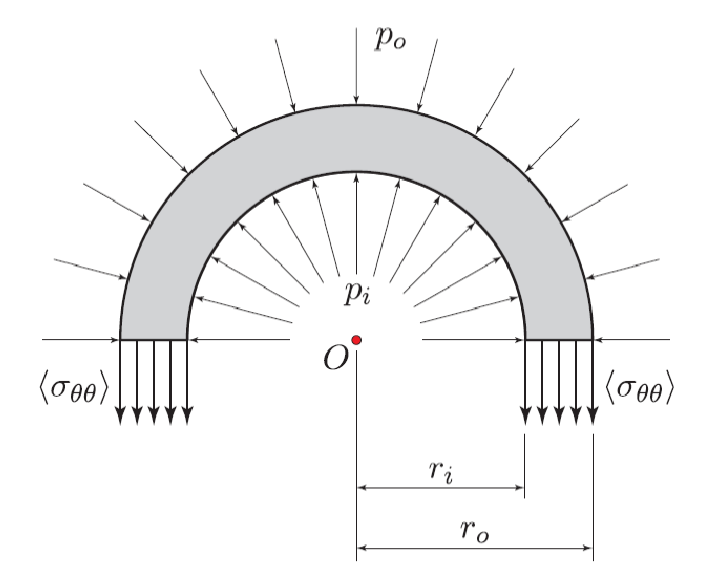
\includegraphics[scale=0.5]{cylindricaltissueslice.png}

\subsection{Analytical analysis fot thick-walled cylinders}

Stress equilibrium (Balance of Momentum)
\begin{equation}
    \nabla \cdot \bm{\sigma} + \vec{f} = \rho \frac{D^2\vec{u}}{Dt^2}
\end{equation}
Stress equilibrium in a thick-walled cylinder
\begin{equation}
    P = \int_{r_i}^{r_o}(\sigma_{\theta\theta}-\sigma_{rr})\frac{dr}{r}
\end{equation}
NeoHookean formulation for the Cauchy Stress in a thick-walled cylinder
\begin{align}
    \sigma_{rr} & = 2c_1\lambda_{\theta}^{-2}\lambda_z^{-2}-p \\
    \sigma_{\theta\theta} & = 2c_1\lambda_{\theta}^{2}-p \\
    \sigma_{zz} & = 2c_1\lambda_z^{2}-p
\end{align}
with
\begin{align}
    \lambda_{\theta} & = \frac{r}{R}\\
    r & = \sqrt{\lambda_{\theta, i}^2R_i^2+\frac{R^2-R_i^2}{\lambda_z}}
\end{align}

\subsection{The Finite Element Method}

\section{Other biomechanical applications}

\end{document}